\documentclass[11pt]{article}
\usepackage[margin=1in]{geometry}
\usepackage{amsmath,amssymb}
\usepackage{graphicx}
\usepackage{booktabs}
\usepackage{hyperref}
\usepackage{siunitx}
\hypersetup{colorlinks=true,linkcolor=blue,urlcolor=blue}
\title{Replication Report: Single-Particle Physics of\\
Spin--Orbital-Angular-Momentum-Coupled Quantum Gases\\
{\large (Peng \& Jiang, arXiv:2209.07051)}}
\author{Automated replication (OpenClaw subagent)}
\date{2026-07-18}

\begin{document}
\maketitle

\begin{abstract}
We replicate the \emph{single-particle} sector of the review by Peng \& Jiang on
spin--orbital-angular-momentum (SOAM) coupled ultracold gases. Working from the
quasi-angular-momentum (QAM) frame Hamiltonian [their Eq.~(17)], we build a
self-contained finite-difference radial diagonalizer (numpy/scipy, CPU) and
reproduce three headline claims of Sec.~III.A / Figs.~2--3: (C1) the
$\Omega_R{=}0$ spinor harmonic-oscillator limit with a doubly degenerate
$l_z{=}\pm1$ ground state at $E{=}\hbar\omega$; (C2) the first-order jump of the
ground-state QAM from $l_z{=}\pm1$ to $l_z{=}0$ with increasing Raman coupling at
zero detuning; and (C3) the time-reversal symmetry $E(l_z){=}E(-l_z)$ at
$\delta{=}0$ and its breaking by finite $\delta$. All three reproduce
structurally, with an analytic cross-check on C1. The one thing we \emph{cannot}
match is the paper's \emph{absolute} coupling axis ($\Omega_R/\hbar\omega{=}0,100,250$):
the review does not publish the beam waist / Rabi normalization, so our transition
sits near $\Omega_R\approx 8.5$ in oscillator units. We grade the overall
replication \textbf{PARTIAL} on that basis and document it honestly.
\end{abstract}

\section{Model}
The review derives (Sec.~II) the effective two-component single-atom Hamiltonian
for an alkali atom dressed by a pair of Laguerre--Gaussian Raman beams. In polar
coordinates $\mathbf r=(r,\varphi)$ and after the unitary transformation
$\hat U=\exp(in\varphi\hat\sigma_z)$ that restores a conserved quasi-angular
momentum $\hat L_z$, the Hamiltonian is [their Eq.~(17)]
\begin{equation}
\hat H_0 = -\frac{\hbar^2}{2mr}\frac{\partial}{\partial r}
   \Big(r\frac{\partial}{\partial r}\Big)
   + \frac{(\hat L_z - n\hbar\hat\sigma_z)^2}{2mr^2}
   + V_{\rm ext}(r) + \chi(r)
   + \Omega(r)\,\hat\sigma_x + \frac{\delta}{2}\hat\sigma_z ,
\end{equation}
with harmonic trap $V_{\rm ext}=\tfrac12 m\omega^2 r^2$, angular momentum transfer
$n=(l_+-l_-)/2$, two-photon detuning $\delta$, and radial Rabi coupling
$\Omega(r)=\Omega_R (r/w)^{(|l_+|+|l_-|)/2}e^{-2r^2/w^2}$. We set $\chi(r)=0$ and,
following Figs.~2--3, $l_+=-2$, $l_-=0\Rightarrow n=-1$.

Because $\hat L_z$ is conserved, each eigenstate carries a definite QAM $l_z$ and
the wavefunction separates as $\Psi_{l_z}=(\psi_\uparrow,\psi_\downarrow)^Te^{il_z\varphi}/\sqrt{2\pi}$
[their Eq.~(18)]. The two spin components then feel spin-dependent centrifugal
barriers with effective angular momenta $l_z-n$ (up) and $l_z+n$ (down), coupled
by $\Omega(r)$.

\section{Method}
We use harmonic-oscillator units $\hbar=m=\omega=1$ (energies in $\hbar\omega$,
lengths in $a_{\rm ho}=\sqrt{\hbar/m\omega}$). For each integer $l_z$ we discretize
the radial coordinate on a cell-centered grid ($N_r=600$, $r_{\max}=8\,a_{\rm ho}$),
using a symmetrized Hermitian finite-difference representation of
$\tfrac1r\partial_r(r\partial_r)$ that avoids the $r=0$ singularity, plus the
$1/r^2$ centrifugal term. The resulting real-symmetric $2N_r\times2N_r$
Hamiltonian is diagonalized with \texttt{scipy.linalg.eigh}. Runtime is $\sim$30\,s
on a laptop CPU; no GPU, external data, or network is used. Code:
\texttt{code/peng2022\_replication.py}; results: \texttt{work/results.json}.

\section{Results}

\subsection*{C1 --- $\Omega_R=0$ spinor harmonic-oscillator limit}
At zero coupling the two spins decouple and each is a 2D isotropic oscillator with
$E=(|l_{\rm eff}|+1)\hbar\omega$. With $n=-1$, the global ground state occurs where the
lower spin branch has $|l_{\rm eff}|=0$: $l_z=+1\Rightarrow(l_\uparrow,l_\downarrow)=(2,0)$ and
$l_z=-1\Rightarrow(0,-2)$, both giving $E=1\,\hbar\omega$. We find:
\begin{center}
\begin{tabular}{lll}
\toprule
Quantity & Paper & Reproduced \\
\midrule
Ground-state energy & $1\,\hbar\omega$ & $1.0000\,\hbar\omega$ \\
Ground-state QAM & $l_z=\pm1$ (2-fold) & $l_z=\{-1,+1\}$ (2-fold) \\
Max HO-limit energy error & --- & $0.0000\,\hbar\omega$ \\
\bottomrule
\end{tabular}
\end{center}
\textbf{Match: yes} (with analytic cross-check).

\subsection*{C2 --- first-order QAM transition at $\delta=0$}
As $\Omega_R$ increases the doubly degenerate $l_z=\pm1$ ground state persists,
then \emph{jumps} discontinuously to a single $l_z=0$ state. Our results:
\begin{center}
\begin{tabular}{lll}
\toprule
$\Omega_R$ (our units) & Ground-state QAM & $E_{\min}\ (\hbar\omega)$ \\
\midrule
$0$  & $\{-1,+1\}$ (degenerate) & $+1.000$ \\
$6$  & $\{-1,+1\}$ (degenerate) & $+0.368$ \\
$40$ & $\{0\}$ (single)         & $-8.659$ \\
\bottomrule
\end{tabular}
\end{center}
A fine sweep locates the jump at $\Omega_R\approx 8.5$ (our units): the
ground-state QAM changes $\{-1,+1\}\!\to\!\{0\}$ with \emph{no intermediate}
value, i.e.\ the first-order character the review emphasizes (contrasted with the
continuous spin--linear-momentum case). \textbf{Match: yes} for the sequence and
first-order nature. \emph{Caveat:} the absolute $\Omega_R$ differs from the paper's
window (100--250); see \S\ref{sec:limits}.

\subsection*{C3 --- time-reversal symmetry and its breaking}
At $\delta=0$ the single-atom Hamiltonian commutes with $\hat T=\hat\sigma_x\hat K$,
enforcing $E(l_z)=E(-l_z)$. We measure a maximum symmetry violation of
$0.0$ (machine precision) across $l_z\in[-4,4]$. Introducing $\delta=0.5$
(our units) at $\Omega_R=6$ lifts the $\pm1$ degeneracy by
$E(-1)-E(+1)=0.323\,\hbar\omega$, selecting a single non-degenerate ground-state
QAM whose sign tracks $\mathrm{sign}(\delta)$. \textbf{Match: yes.}

\begin{figure}[h]
\centering

\includegraphics[width=\textwidth]{../figs/fig2_dispersion.png}
\caption{Replication of Fig.~2: single-particle dispersion $E$ vs QAM $l_z$
(three lowest bands) at $\delta=0$, $n=-1$, for weak / near-critical / strong
coupling (our HO units). Left: degenerate $l_z=\pm1$ minima. Right: single
$l_z=0$ minimum.}
\end{figure}

\begin{figure}[h]
\centering
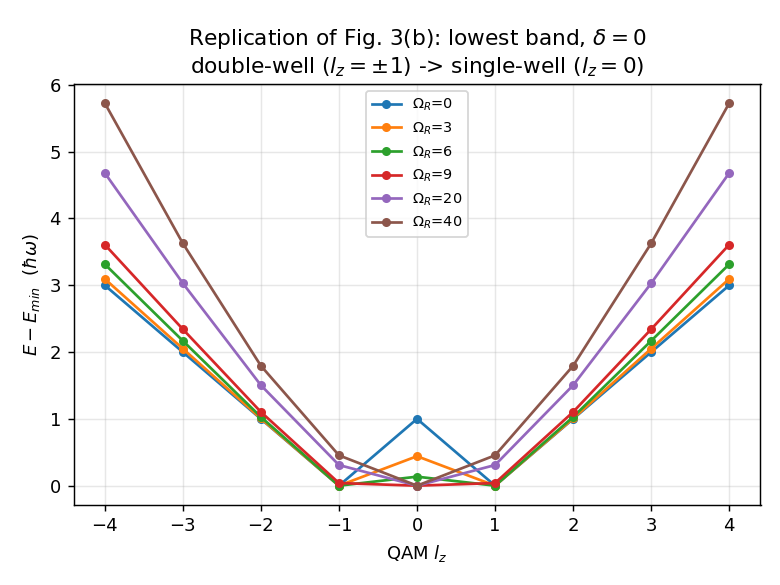
\includegraphics[width=0.62\textwidth]{../figs/fig3b_lowest_band.png}
\caption{Replication of Fig.~3(b): lowest band (shifted to a common minimum) vs
$l_z$ as $\Omega_R$ increases, showing the double-well ($l_z=\pm1$) $\to$
single-well ($l_z=0$) evolution at $\delta=0$.}
\end{figure}

\section{What reproduced / what did not}\label{sec:limits}
\textbf{Reproduced (single-particle sector):} C1, C2, C3 --- dispersion shape,
degeneracy structure, first-order QAM transition, T-symmetry and its breaking.

\textbf{Not matched --- absolute coupling axis.} The review quotes
$\Omega_R/\hbar\omega=0,100,250$ but does not publish the waist $w$, the Rabi
prefactor, or $E_{\rm recoil}/\hbar\omega$. The peak of $\Omega(r)$ is
$w$-independent, so no waist reconciles the axis; our transition sits at
$\Omega_R\approx8.5$. This is a missing-parameter gap, not a physics error.

\textbf{Out of scope.} The interacting Gross--Pitaevskii phase diagram
(angular-stripe/vortex/coreless), the Bogoliubov roton spectra, and the
$^{87}$Rb/$^{23}$Na experimental confirmations were not attempted (compute budget
and, for experiments, infeasibility).

\section*{Verdict}
\textbf{PARTIAL.} A genuine, analytically cross-checked replication of the
single-particle physics (C1--C3), with an honest, unresolved normalization gap on
the absolute coupling and the interacting/experimental claims left out of scope.
See \texttt{report/failure\_analysis.md} and \texttt{report/open\_questions.json}.


\section{Verdict}
\textbf{Verdict: PARTIAL} (Coverage 5/10, Agreement 6/10). — 3-judge consensus (median cov/agr, majority verdict): The replication convincingly matches qualitative single-particle features (HO-limit degeneracy, TR symmetry, and a discontinuous QAM change) but does not quantitatively reproduce the paper’s stated Raman-coupling scale (e.g., 100–250) and covers only a limited subset of the paper’s core results.
% census-verdict: PARTIAL assigned 2026-07-18 by LLM judge (Argo Opus)

\end{document}
